\frame{
\begin{tikzpicture}[remember picture,overlay]
\fill[blue1]
(current page.north west) rectangle ([xshift=12.cm,yshift=-10.cm]current page.east|-{pic cs:end});
\end{tikzpicture}

\begin{textblock}{0.9}(0.05,0.08)
\centering
\Huge{
\textcolor{white}{Measuring the volume fraction of \textbf{dynamic} granular systems}}\\
\end{textblock}

\begin{textblock}{0.9}(0.05,0.34)
	\centering
	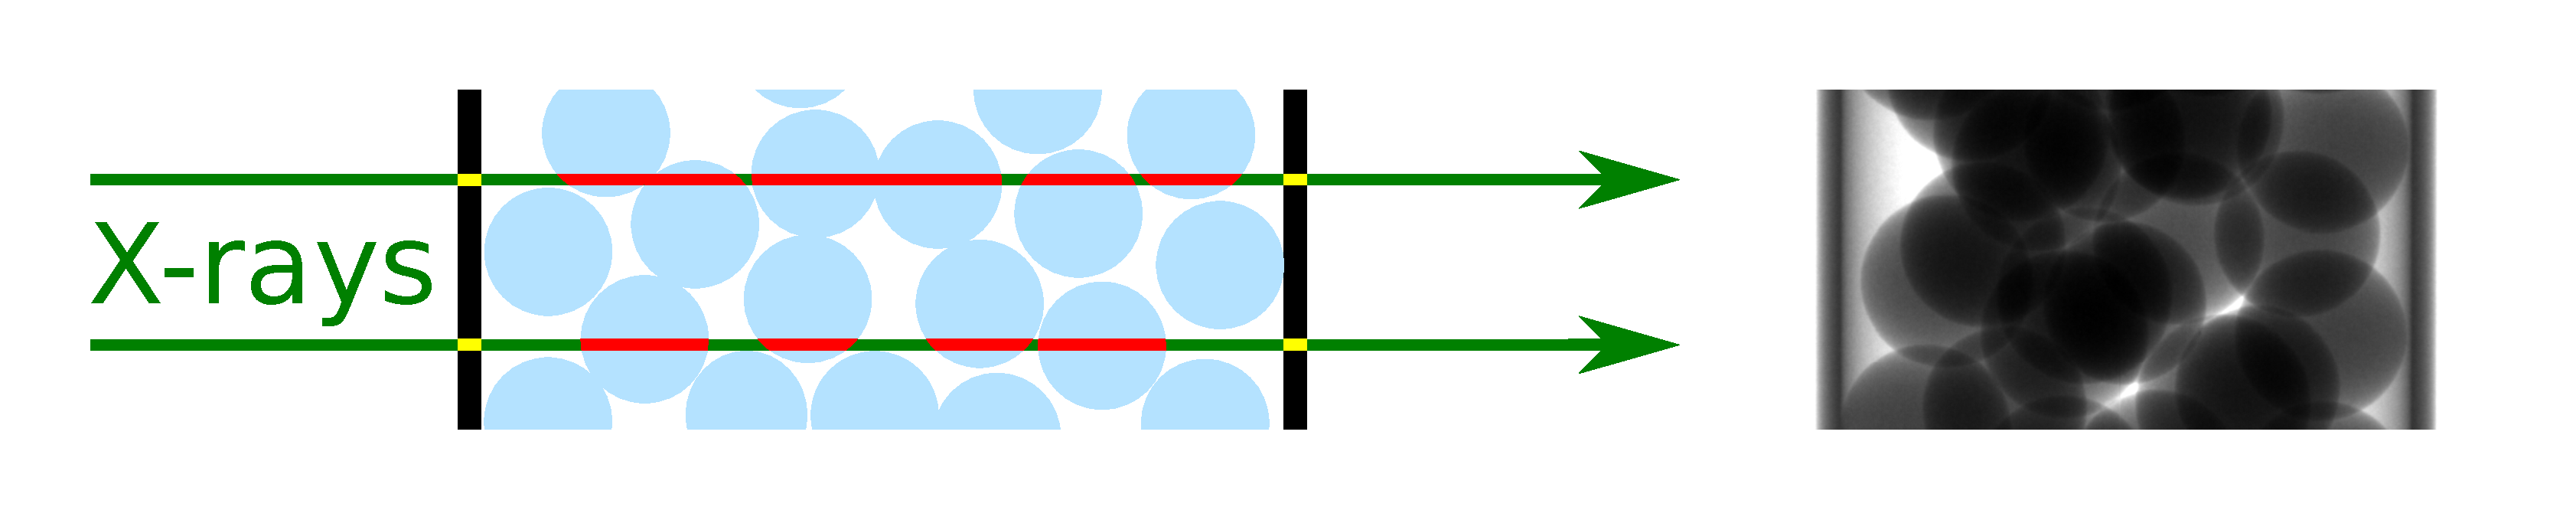
\includegraphics[width=0.8\textwidth]{Sources/beam_hardening/2beams_attenuation_marked.pdf}
\end{textblock}

\begin{textblock}{0.9}(0.05,0.65)
\visible<1->{
\centering
\Huge{
	\textcolor{white}{Correction of beam hardening \\
		in X-ray radiograms}}}
\end{textblock}

\begin{textblock}{0.9}(0.05,0.9)
	\visible<1->{
	\centering
	{
	\textcolor{white}{
		Baur \textit{et al}, \textit{Rev.\ Sci.\ Instrum.}\ (2019)\\
		In collaboration with Norman Uhlmann, Fraunhofer EZRT}}}
\end{textblock}
}


%% ------------------ ATTENUATION OF X-RAYS -----------------------
\frame{
\begin{tikzpicture}[remember picture,overlay]
\fill[blue1]
(current page.north west) rectangle ([xshift=0.32\paperwidth,yshift=0.33\paperheight]current page.west|-{pic cs:end});
\end{tikzpicture}

\begin{textblock}{0.5}(0.02,0.03)
	\textcolor{white}{
		\Large Attenuation of X-rays}
\end{textblock}

\begin{textblock}{0.45}(0.5,0.1)
\centering
Beer-Lambert's law\\[0.1cm]
\only<1,2,3,4,5>{
$\textcolor{red}{I(x)} = \textcolor{blue}{I_0} \exp(- \mu\, x)$}
\only<6,7>{
	$\xcancel{\textcolor{red}{I(x)} = \textcolor{blue}{I_0} \exp(- \mu\, x)}$}\\[0.1cm]
\only<6,7>{
$\textcolor{red}{I(x)} = 
	\textcolor{blue}{I_0} \exp(- \textcolor{darkgreen}{\mu_\text{eff}(x)}\, x)$
}
\end{textblock}


\begin{textblock}{0.45}(0.03,0.14)
	\centering
	\only<1> {%% image of beam through material
	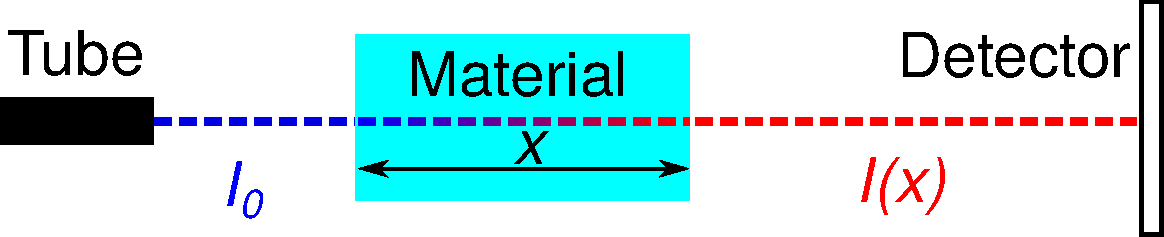
\includegraphics[width=\textwidth]
	{Sources/beam_hardening/beam_through_material.pdf}}
	\only<2>{
	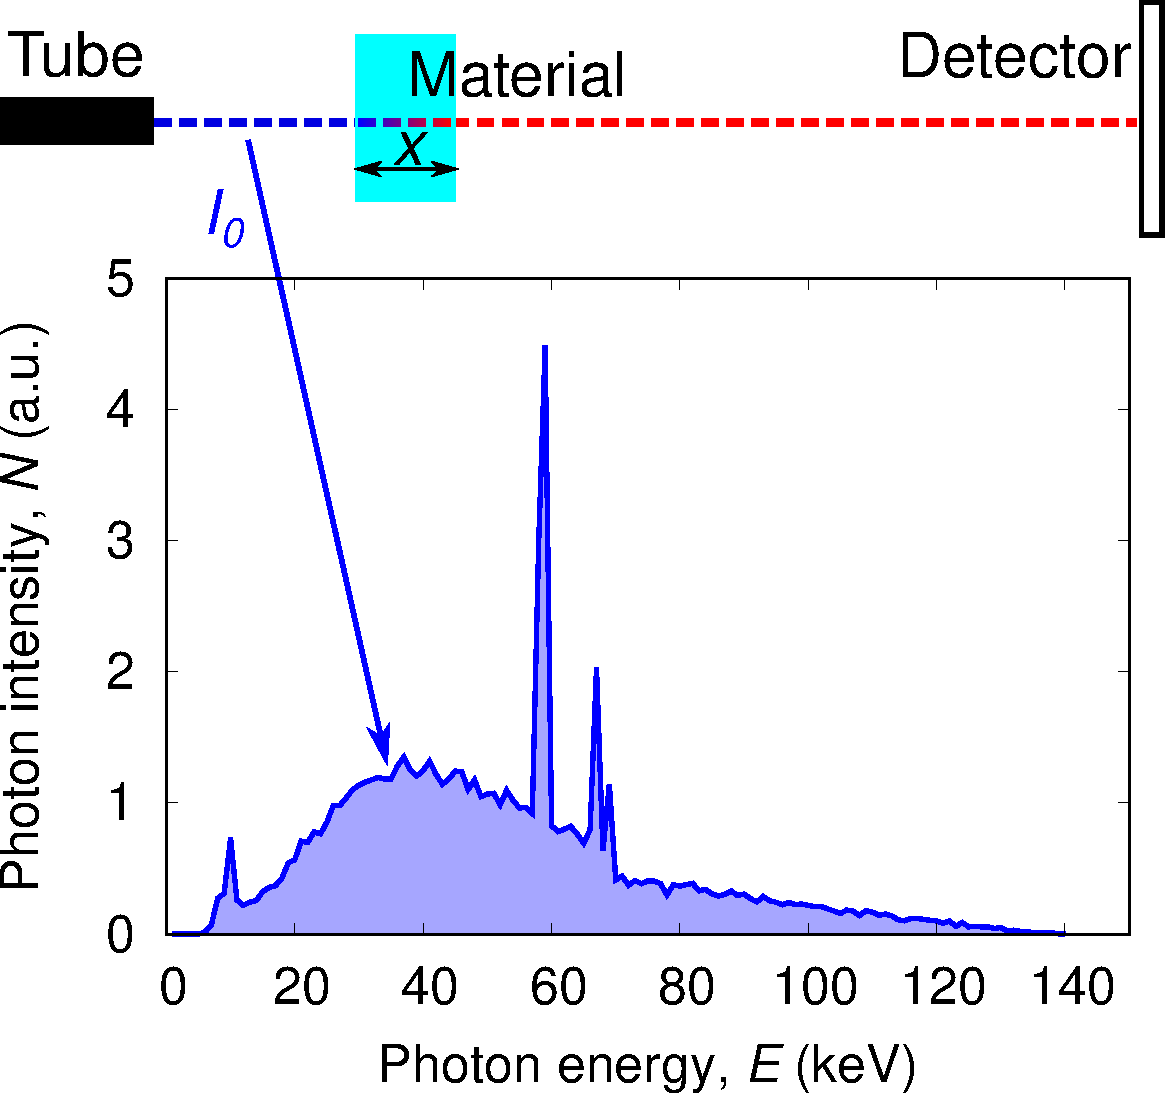
\includegraphics[width=\textwidth]
	{Sources/beam_hardening/x-ray_spectrum_N0_short.pdf}}
	\only<3>{
	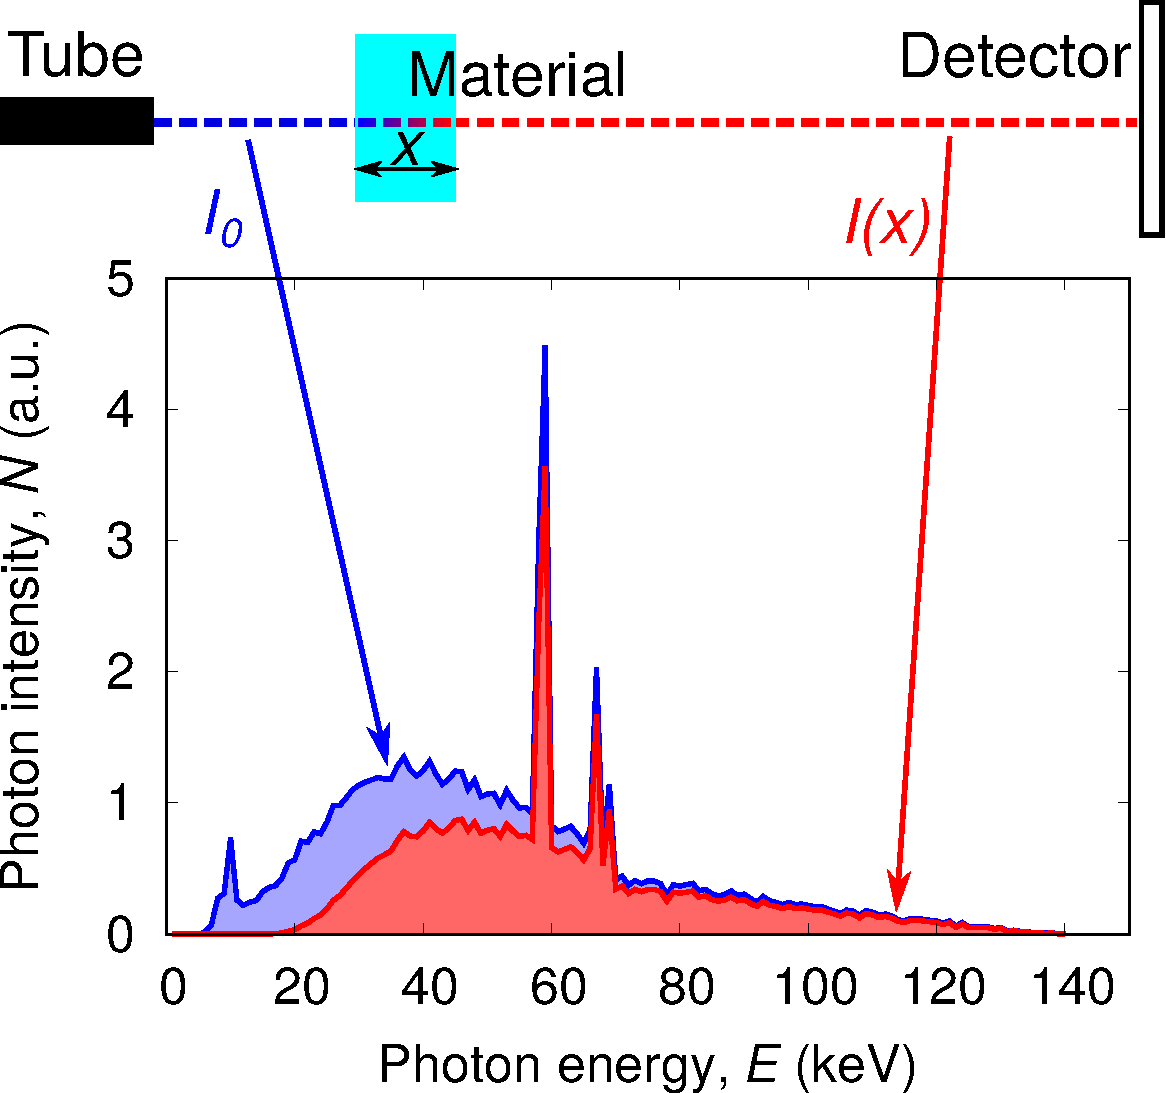
\includegraphics[width=\textwidth]
	{Sources/beam_hardening/x-ray_spectra_beam_hardening_step1.pdf}}
	\only<4>{
	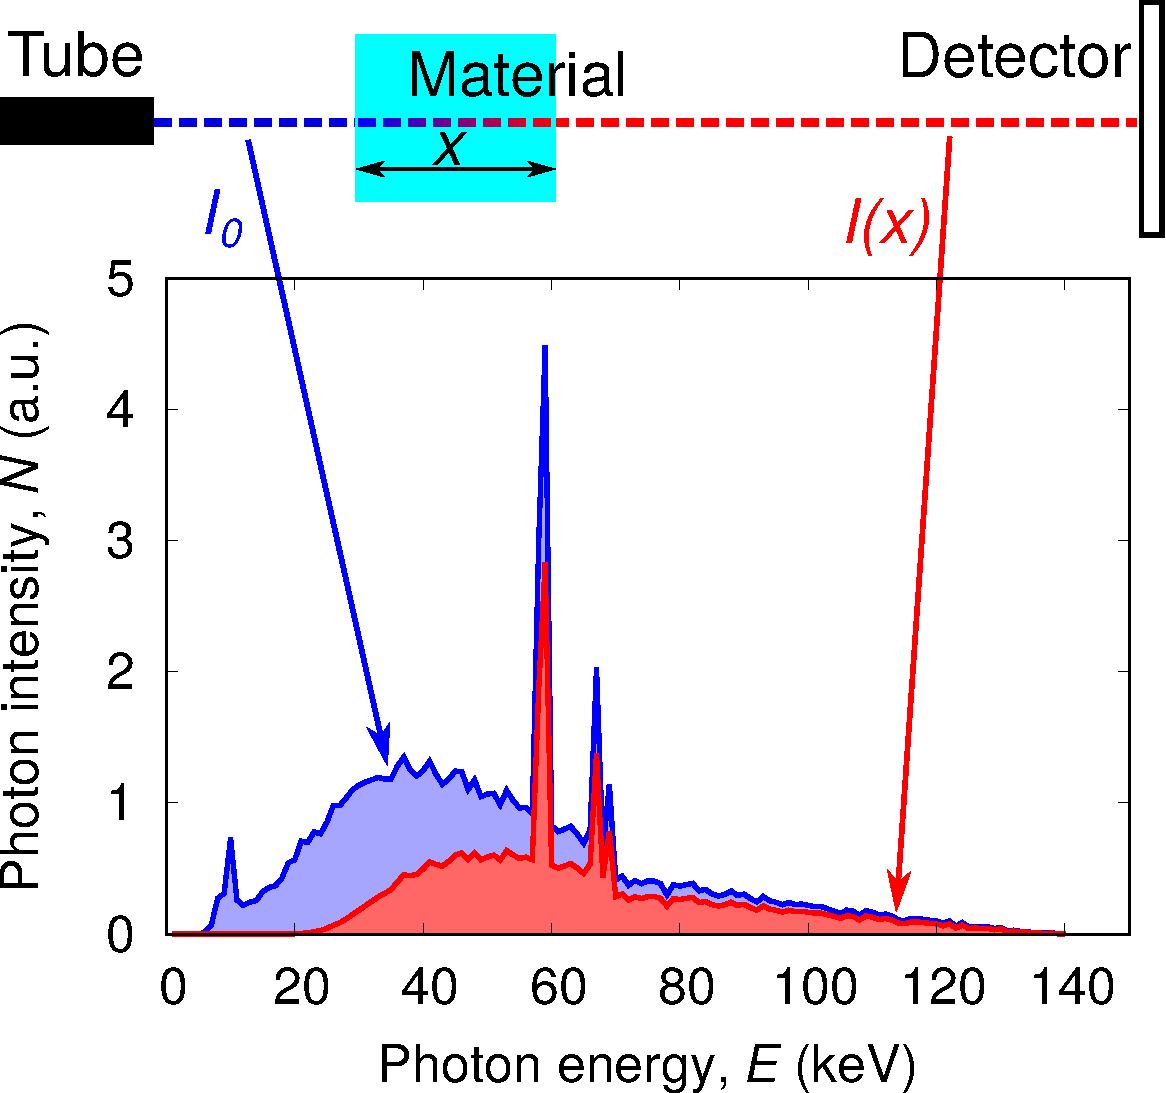
\includegraphics[width=\textwidth]
	{Sources/beam_hardening/x-ray_spectra_beam_hardening_step2.pdf}}
	\only<5,6,7>{
	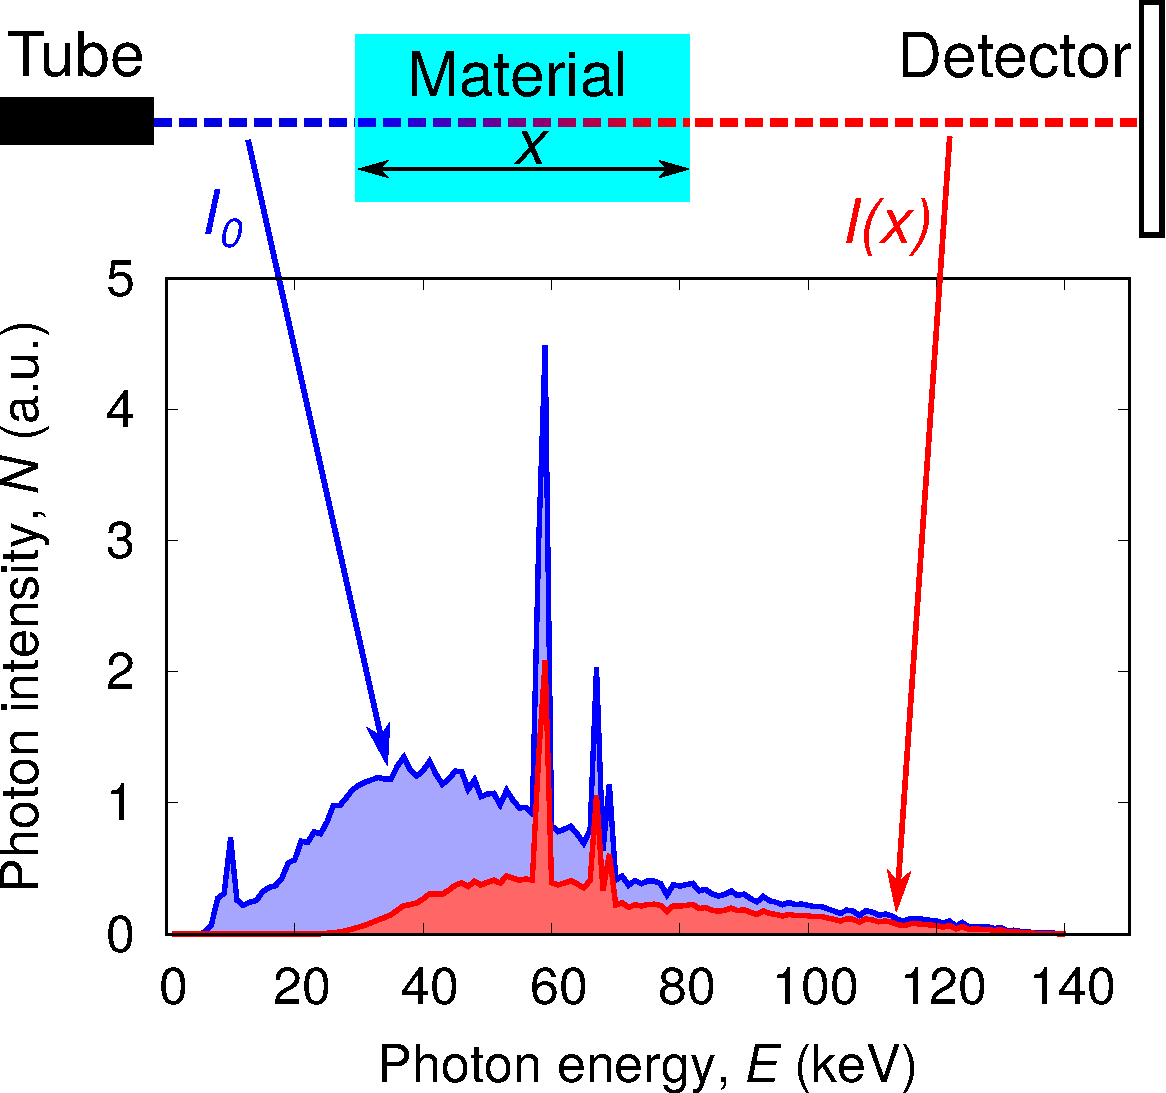
\includegraphics[width=\textwidth]
	{Sources/beam_hardening/x-ray_spectra_beam_hardening.pdf}}
\end{textblock}
\begin{textblock}{0.45}(0.035,0.36)
	\centering
	\visible<6->{
	\colorbox{red}{Beam hardening}}
\end{textblock}

\begin{textblock}{0.48}(0.5,0.3)
	\visible<7->{
	\includegraphics[width=\textwidth]
	{Sources/beam_hardening/attenuation_boro_glass_140kV.pdf}}
\end{textblock}

\begin{textblock}{0.3}(0.66,0.35)
	\centering
	\visible<7->{
	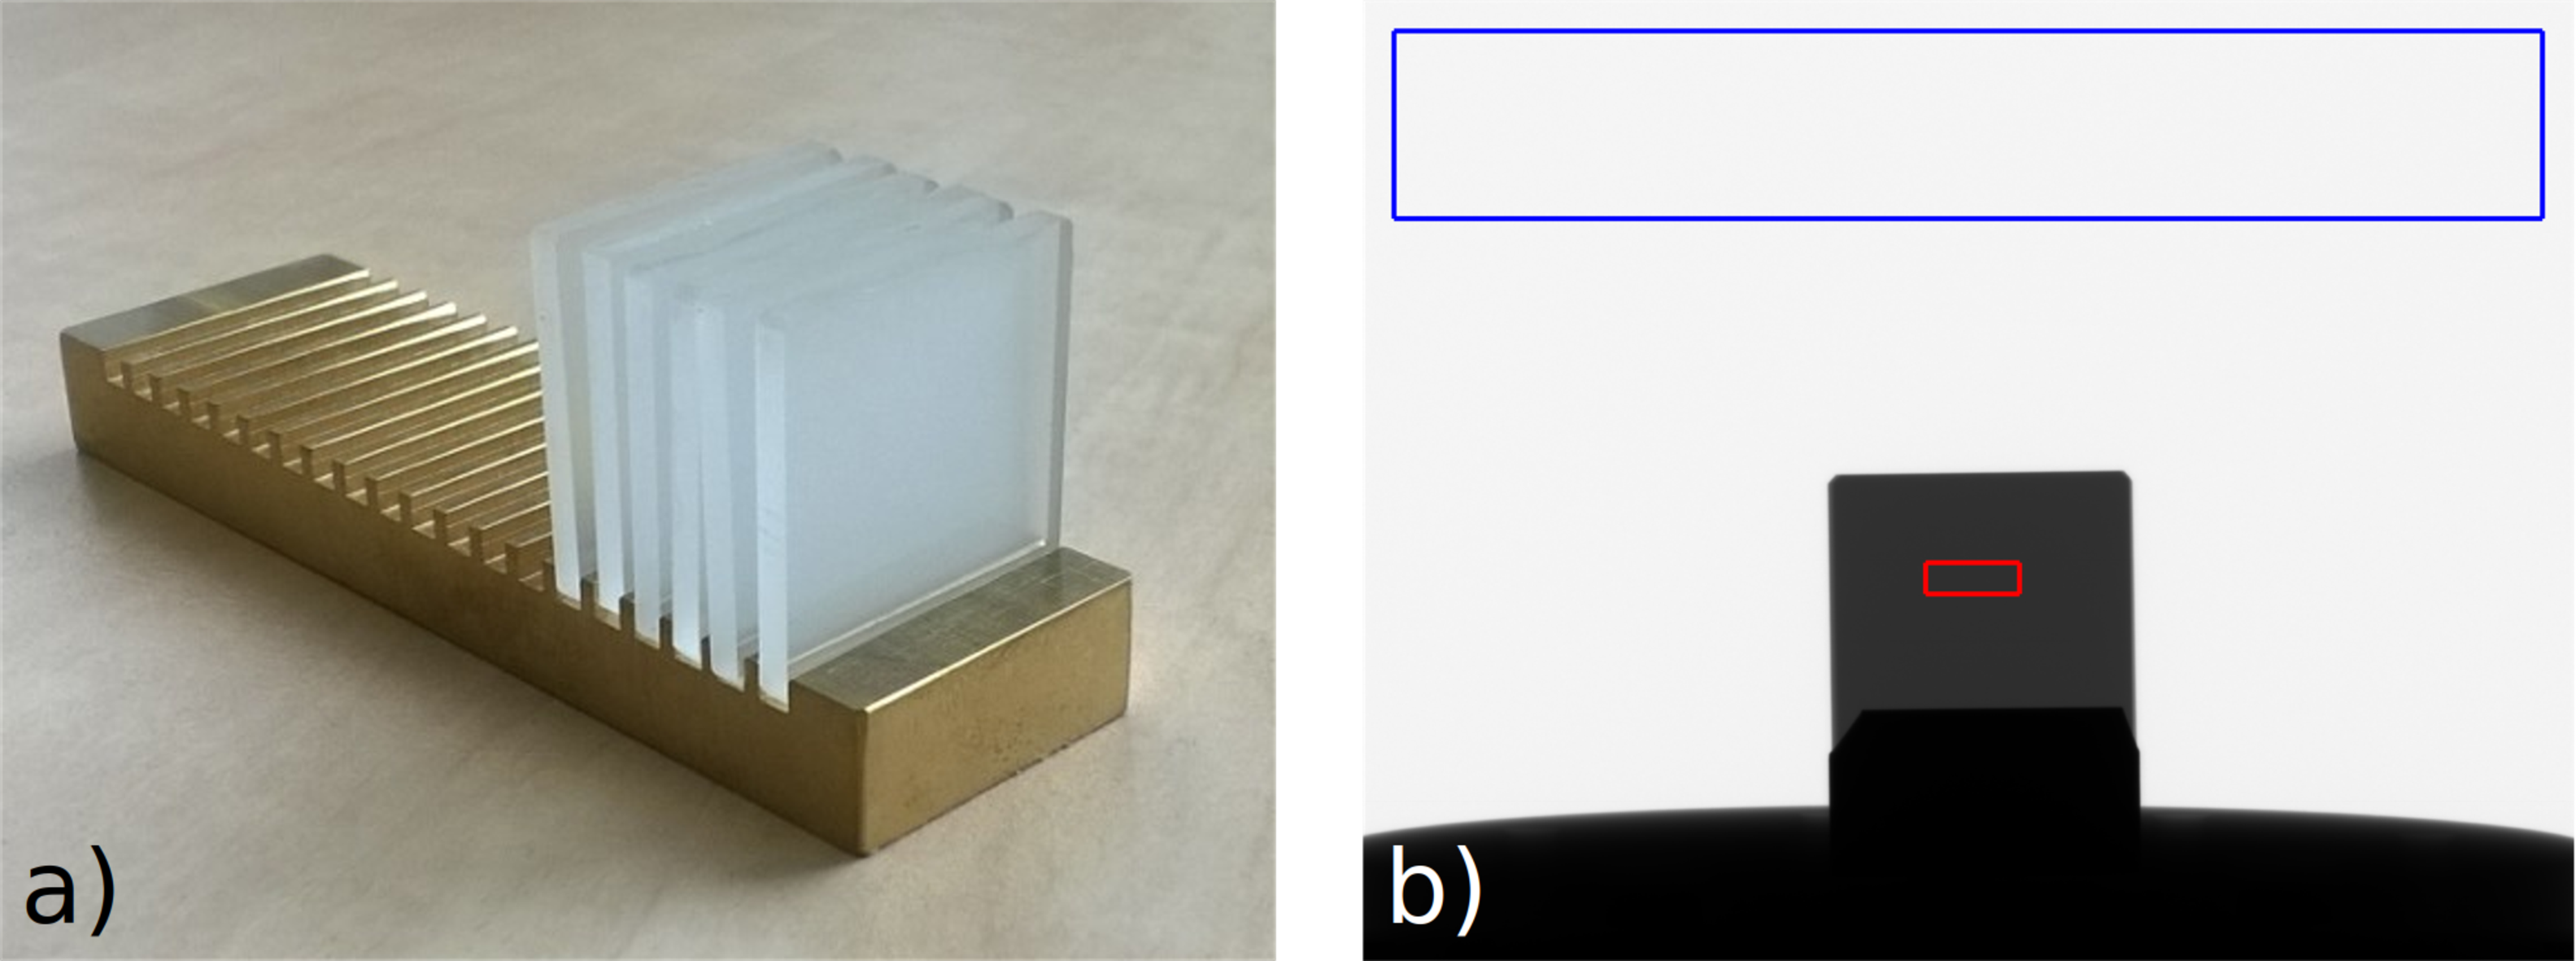
\includegraphics[width=\textwidth]
	{Sources/beam_hardening/Plates_on_slide_horizontal.pdf}}
\end{textblock}
}



%% ------------------ ATTENUATION OF X-RAYS -----------------------
\frame{
	\begin{tikzpicture}[remember picture,overlay]
	\fill[blue1]
	(current page.north west) rectangle ([xshift=0.32\paperwidth,yshift=0.33\paperheight]current page.west|-{pic cs:end});
	\end{tikzpicture}
	
	\begin{textblock}{0.5}(0.02,0.03)
		\textcolor{white}{
			\Large Attenuation of X-rays}
	\end{textblock}
	
	\begin{textblock}{0.45}(0.5,0.1)
		\centering
		Beer-Lambert's law\\[0.1cm]
		\visible<1->{
			$\textcolor{red}{I(x)} = \textcolor{blue}{I_0} \exp(- \textcolor{darkgreen}{\mu(E,Z,\rho)}\, x)$
			}
	\end{textblock}
	
	\begin{textblock}{0.48}(0.5,0.3)
		\visible<1->{
			\centering
			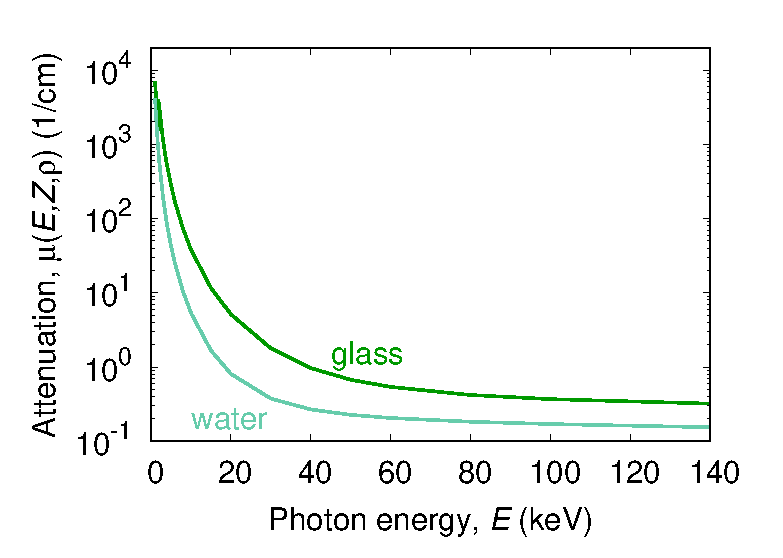
\includegraphics[width=\textwidth]
			{Sources/beam_hardening/Attenuation_vs_energy.eps}}
	\end{textblock}
	\begin{textblock}{0.48}(0.5,0.95)
		\centering
		\visible<1->{\scriptsize{
				Tabulated attenuation coefficients from NIST.gov}}
	\end{textblock}
	
	\begin{textblock}{0.45}(0.03,0.14)
		\centering
		\visible<1->{
			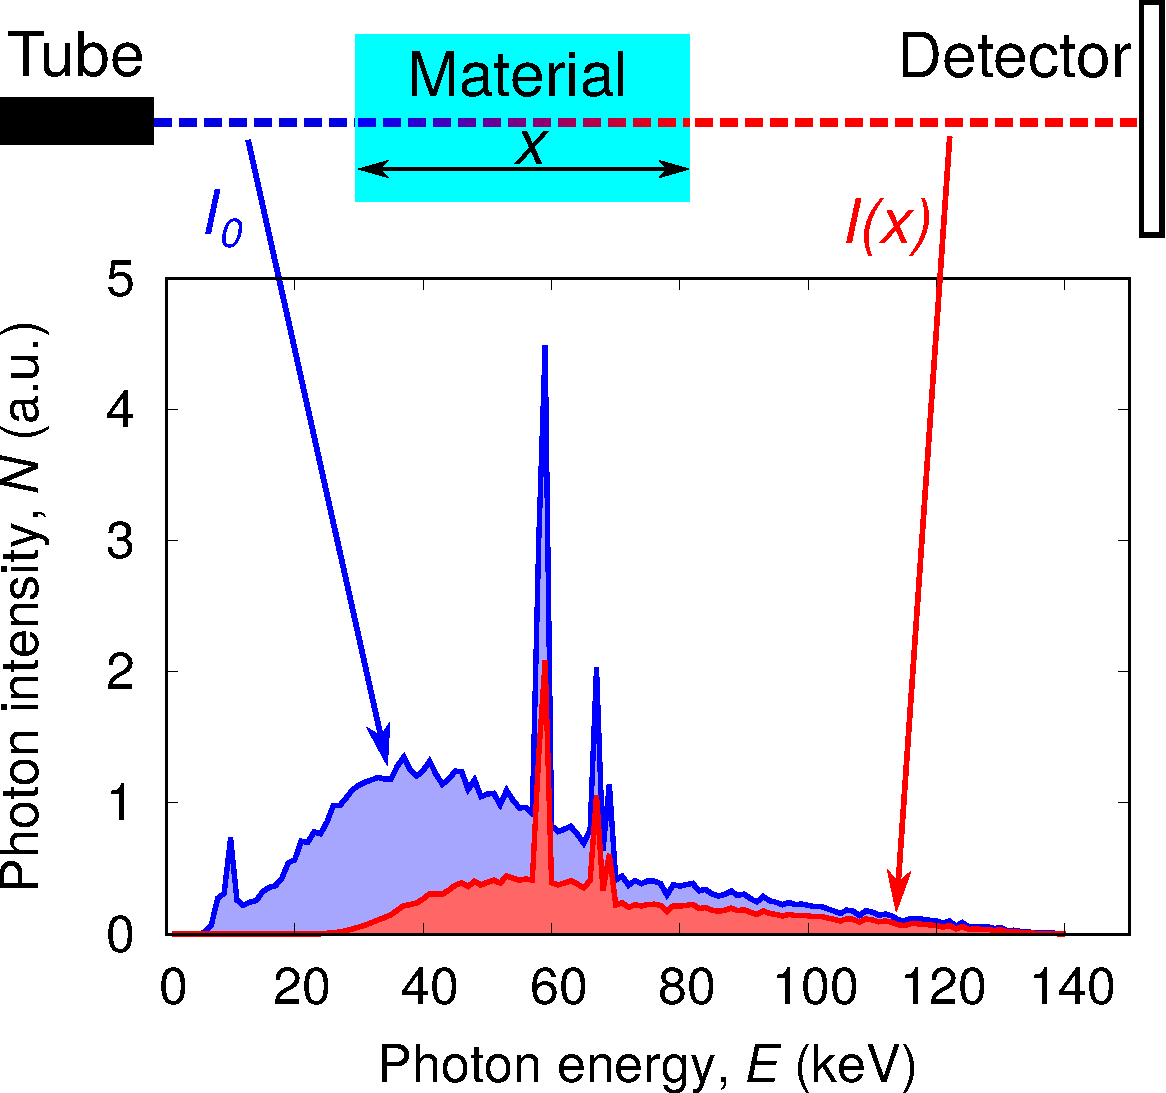
\includegraphics[width=\textwidth]
			{Sources/beam_hardening/x-ray_spectra_beam_hardening.pdf}}
	\end{textblock}
	\begin{textblock}{0.45}(0.035,0.36)
		\centering
		\visible<1->{
			\colorbox{red}{Beam hardening}}
	\end{textblock}	
}




%%%%%%%%%%%%%%%%%%%% Modeling mu_eff %%%%%%%%%%%%%%%%%%%%%%%%%%%%
\frame{
\setlength{\fboxsep}{0pt}
\begin{tikzpicture}[remember picture,overlay]
\fill[blue1]
(current page.north west) rectangle ([xshift=0.29\textwidth,yshift=0.33\textheight]current page.west|-{pic cs:end});
\end{tikzpicture}

\begin{textblock}{0.3}(0.02,0.03)
	\textcolor{white}{
		\Large Modeling of $\mu_\text{eff}(x)$}
\end{textblock}



\begin{textblock}{1.}(0.0,0.03)
	\centering
	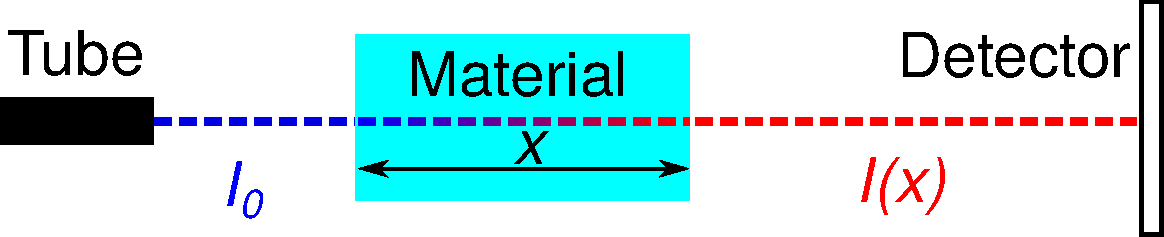
\includegraphics[width=0.4\textwidth]
	{Sources/beam_hardening/beam_through_material.pdf}
\end{textblock}

%% Photon spectrum
\begin{textblock}{0.32}(0.03,0.18)
	\centering
	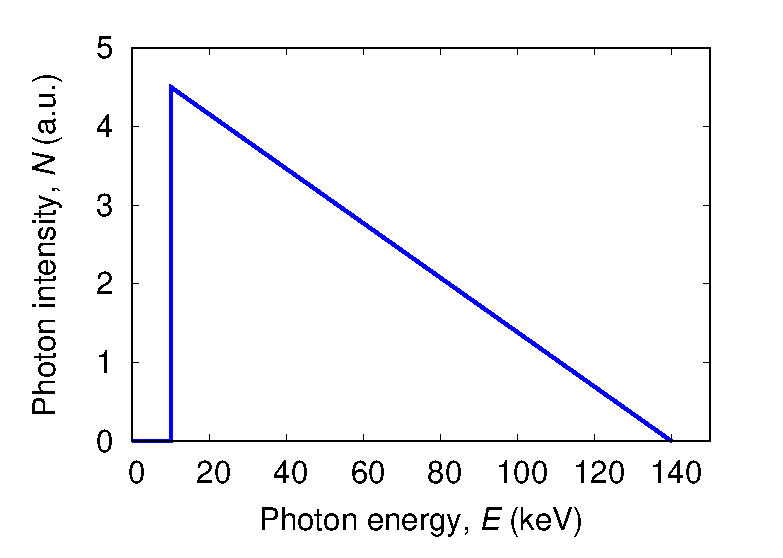
\includegraphics[width=\textwidth]
	{Sources/beam_hardening/linear_spectrum.eps}
\end{textblock}

\begin{textblock}{0.32}(0.07,0.26)
	\centering
%	\hspace{0.5cm}
	\textcolor{blue}{
	\small$N (E) = -a E + b$}
\end{textblock}

%% attenuation data
\begin{textblock}{0.32}(0.345,0.18)
	\centering
	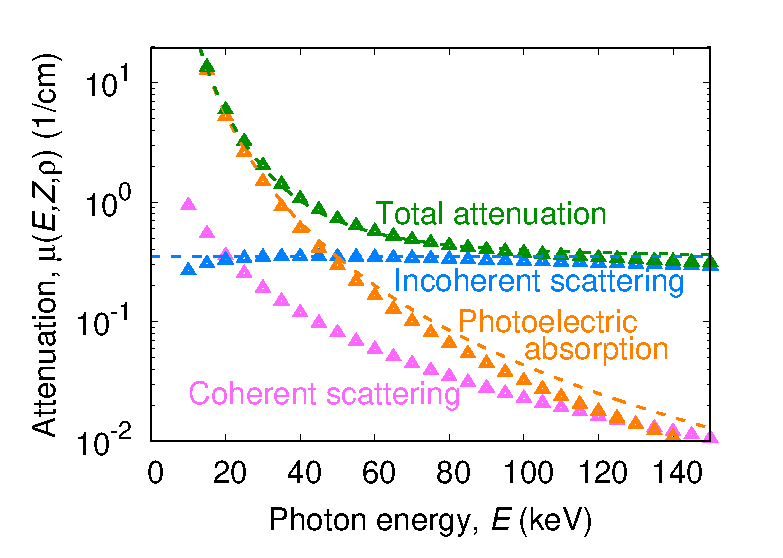
\includegraphics[width=\textwidth]
	{Sources/beam_hardening/XCOM_attenuation.eps}
\end{textblock}

\begin{textblock}{0.32}(0.38,0.26)
	\centering
	\textcolor{darkgreen}{
		\small$\mu (E) = \mu_\text{C} + c E^{-3}\,^{(*)}$}
\end{textblock}

%% detector curve
\begin{textblock}{0.32}(0.67,0.18)
	\centering
	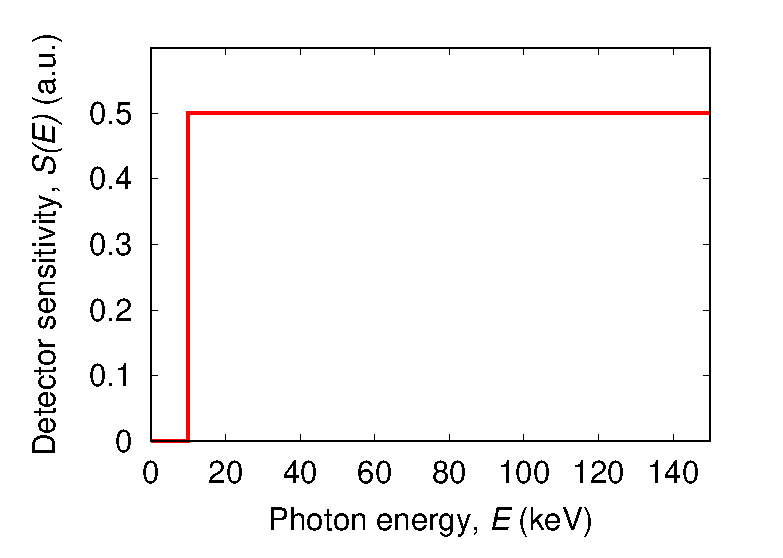
\includegraphics[width=\textwidth]
	{Sources/beam_hardening/detector_const.eps}
\end{textblock}

\begin{textblock}{0.32}(0.68,0.26)
	\centering
	\hspace{0.5cm}
	\colorbox{white}{\textcolor{red}{
		\small$S(E) = S~\Theta(E - E_\text{min})$}}
\end{textblock}

\begin{textblock}{0.5}(0.02,0.6)
	\only<1>{
		\begin{align}
		I(x) &\propto \int \textcolor{blue}{N(E)} \exp\{-
		\textcolor{darkgreen}{\mu(E)} x\} 
		\textcolor{red}{S(E)}~\mathsf{d}E \nonumber\\
		&\textcolor{white}{\propto S \int_{E_\text{min}}^{E_\text{max}}
		(-a E + b) 
		\exp[-(\mu_\text{C} + c E^{-3}) x]~
		\mathsf{d}E}
		\nonumber
		\end{align}
	}
	\visible<2->{
		\begin{align}
		I(x) &\propto \int \textcolor{blue}{N(E)} \exp\{-
		\textcolor{darkgreen}{\mu(E)} x\} 
		\textcolor{red}{S(E)}~\mathsf{d}E \nonumber \\
		&\propto \textcolor{red}{S} \int_{E_\text{min}}^{E_\text{max}}
		(\textcolor{blue}{-a E + b}) 
		\exp\{-(\textcolor{darkgreen}{\mu_\text{C} + c E^{-3}}) x\}~
		\mathsf{d}E 
		\nonumber
		\end{align}
	}
\end{textblock}



\begin{textblock}{0.32}(0.55,0.58)
	\visible<2->{
		\centering
		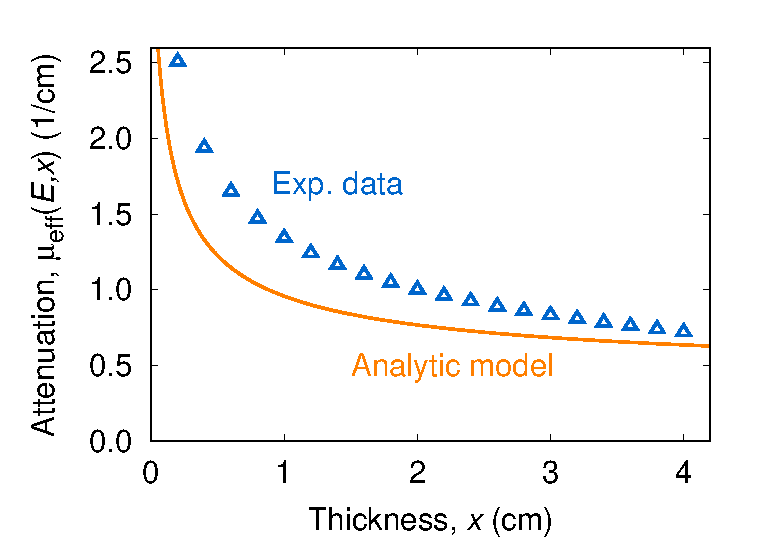
\includegraphics[width=\textwidth]
		{Sources/beam_hardening/attenuation_borosilicate_glass_voltages_first_principle_fit.eps}
	}
\end{textblock}

\begin{textblock}{0.9}(0.02,0.93)
	{\scriptsize
		$(*)$ XCOM supplied by NIST}
\end{textblock}

\begin{textblock}{1.}(0,0)
	\visible<3->{
		
\includegraphics[width=\textwidth]
		{Sources/beam_hardening/cross.pdf}}
\end{textblock}
}



%%%%%%%%%%%%%%%%%% Numerical approach %%%%%%%%%%%%%%%%%%%%%%%%%%%%
\frame{
\begin{tikzpicture}[remember picture,overlay]
\fill[blue1]
(current page.north west) rectangle ([xshift=0.28\textwidth,yshift=0.27\textheight]current page.west|-{pic cs:end});
\end{tikzpicture}

\begin{textblock}{0.23}(0.02,0.03)
	\centering
	\textcolor{white}{
	\Large Numerical approx.\ of 
	$\mu_\text{eff}(x)$}
\end{textblock}



\begin{textblock}{1.}(0.0,0.03)
	\centering
	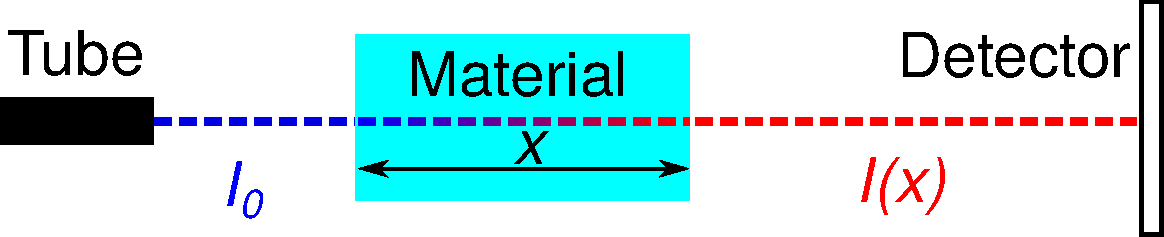
\includegraphics[width=0.4\textwidth]
	{Sources/beam_hardening/beam_through_material.pdf}
\end{textblock}

%% Photon spectrum
\begin{textblock}{0.32}(0.03,0.18)
	\centering
	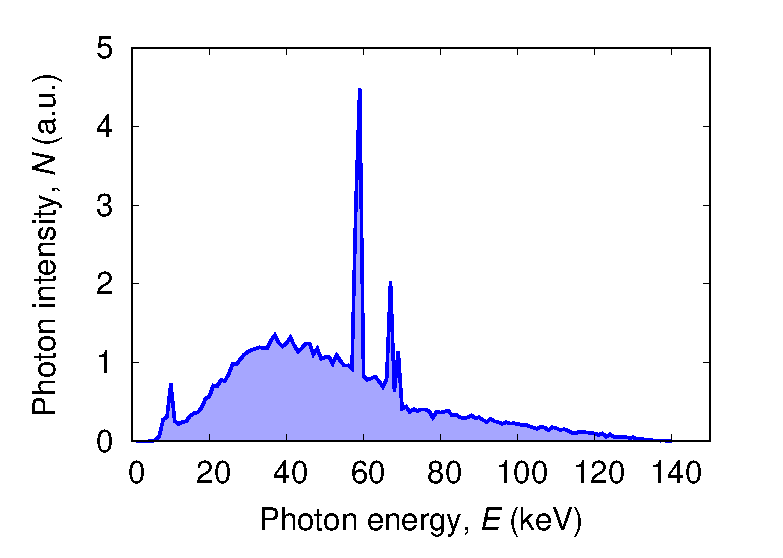
\includegraphics[width=\textwidth]
	{Sources/beam_hardening/N0_initial_spectrum_filled_curves.eps}
\end{textblock}

\begin{textblock}{0.32}(0.045,0.21)
	\centering	
	\textcolor{blue}{
		\small Comet X-ray tube$^{(1)}$}
\end{textblock}

%% attenuation data
\begin{textblock}{0.32}(0.345,0.18)
	\centering
	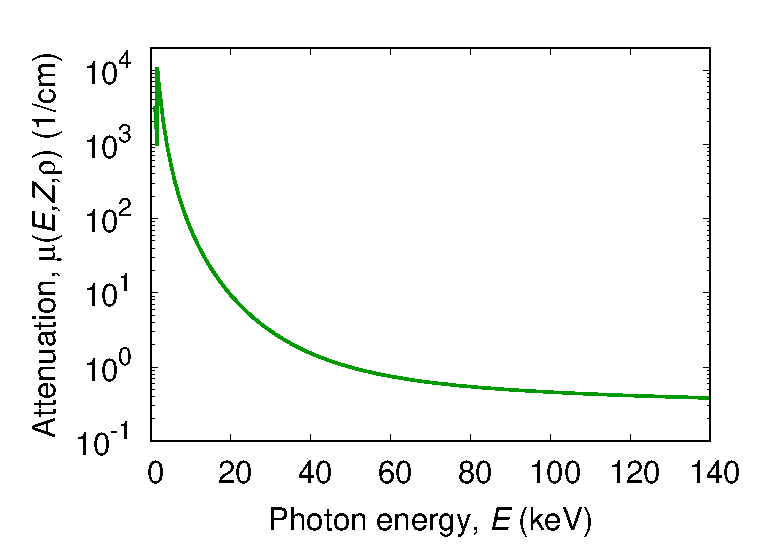
\includegraphics[width=\textwidth]
	{Sources/beam_hardening/Attenuation_vs_energy_Al.eps}
\end{textblock}

\begin{textblock}{0.32}(0.345,0.21)
	\centering
	\textcolor{darkgreen}{
		\small Aluminum$^{(2)}$}
\end{textblock}

%% detector curve
\begin{textblock}{0.32}(0.67,0.18)
	\centering
		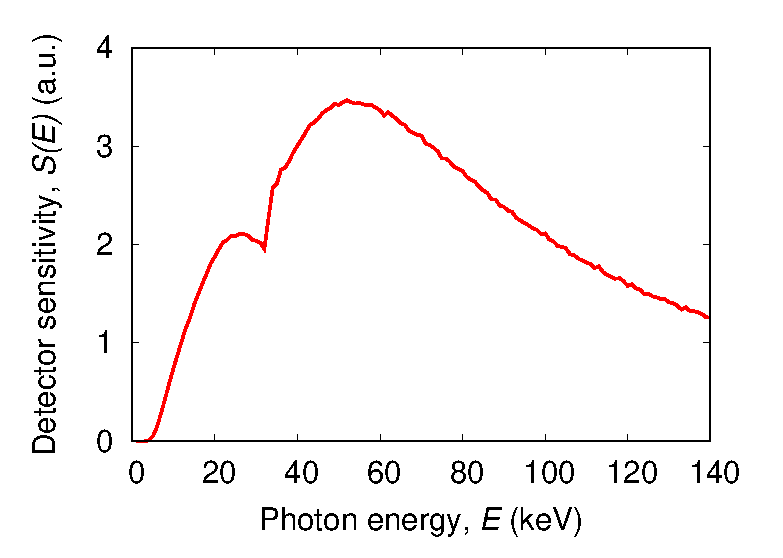
\includegraphics[width=\textwidth]
		{Sources/beam_hardening/Detector_response_0.eps}
\end{textblock}

\begin{textblock}{0.32}(0.67,0.21)
	\centering
	\textcolor{red}{
		\small XEye detector$^{(1)}$}
\end{textblock}


\begin{textblock}{0.5}(0.02,0.6)
	\visible<1->{
	\begin{align}
		I(x) \propto &\int \textcolor{blue}{N(E)} \exp\{-
		\textcolor{darkgreen}{\mu(E)} x\} 
		\textcolor{red}{S(E)}~\mathsf{d}E  \nonumber\\
		&\int \rightarrow \sum \nonumber
	\end{align}
}
\end{textblock}

\begin{textblock}{0.32}(0.55,0.58)
	\visible<2->{
	\centering
	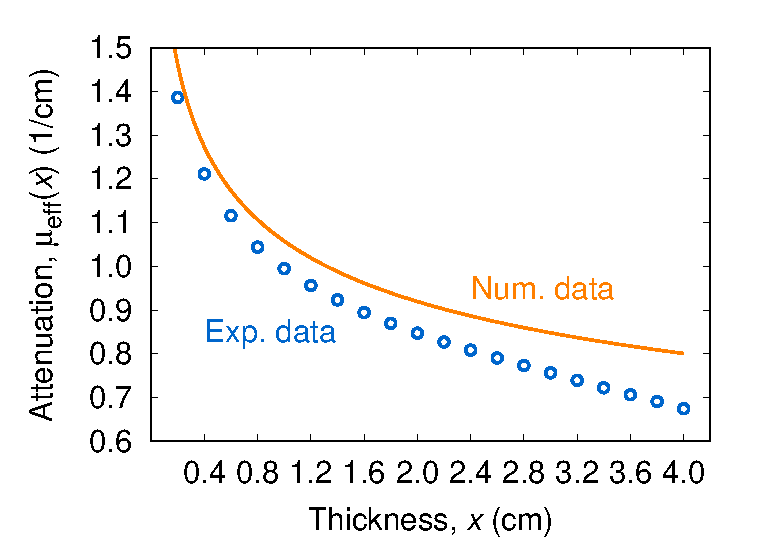
\includegraphics[width=\textwidth]
	{Sources/beam_hardening/mu_eff_140kV_exp_vs_numeric_data_norman.eps}
	}
\end{textblock}

\begin{textblock}{0.9}(0.02,0.9)
{\scriptsize
$(1)$ Supplied by Norman Uhlmann, Fraunhofer EZRT\\
$(2)$ XCOM supplied by NIST}
\end{textblock}

\begin{textblock}{1.}(0,0)
	\visible<3->{
	
\includegraphics[width=\textwidth]
{Sources/beam_hardening/cross.pdf}}
\end{textblock}
}




%% ------------- HEURISTIC MODEL-FUNCTION ------------
\frame{
\begin{tikzpicture}[remember picture,overlay]
\fill[blue1]
(current page.north west) rectangle ([xshift=0.53\textwidth,yshift=0.335\textheight]current page.west|-{pic cs:end});
\end{tikzpicture}

\begin{textblock}{0.5}(0.02,0.03)
	\textcolor{white}{
		\Large Heuristic model functions for $\mu_\text{eff}(x)$}
\end{textblock}

\begin{textblock}{0.39}(0.03,0.1)
	\only<1>{
	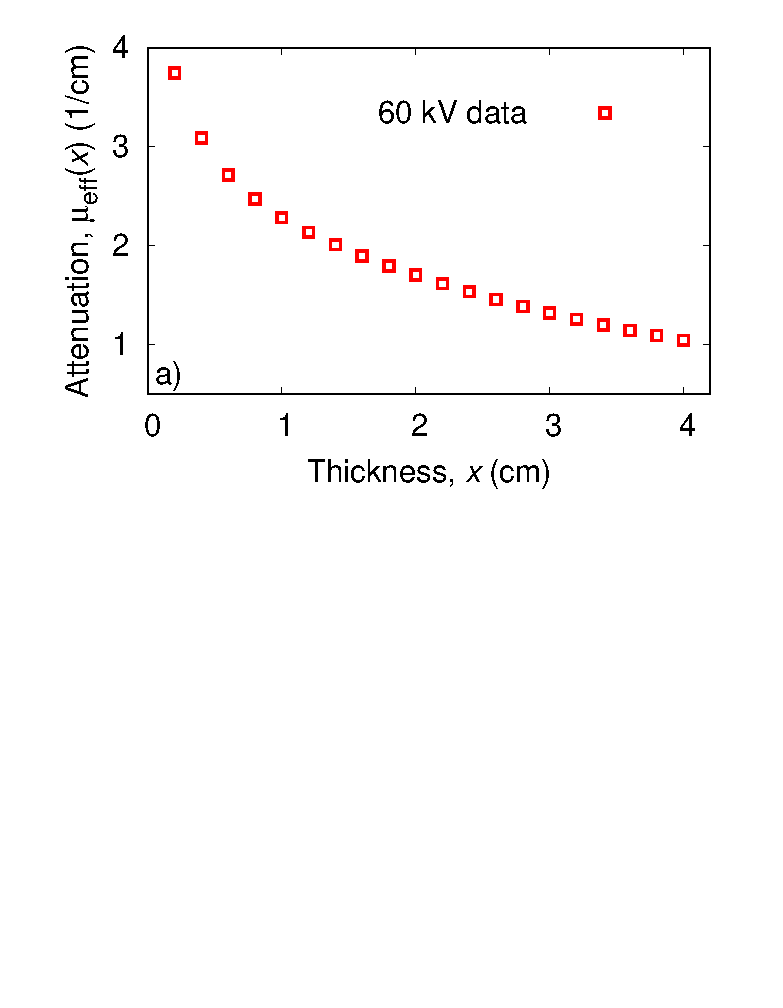
\includegraphics[width=\textwidth]
	{Sources/beam_hardening/borosilicate_glass_60kV_model_comparison_multiplot_1.eps}}
	\only<2>{
	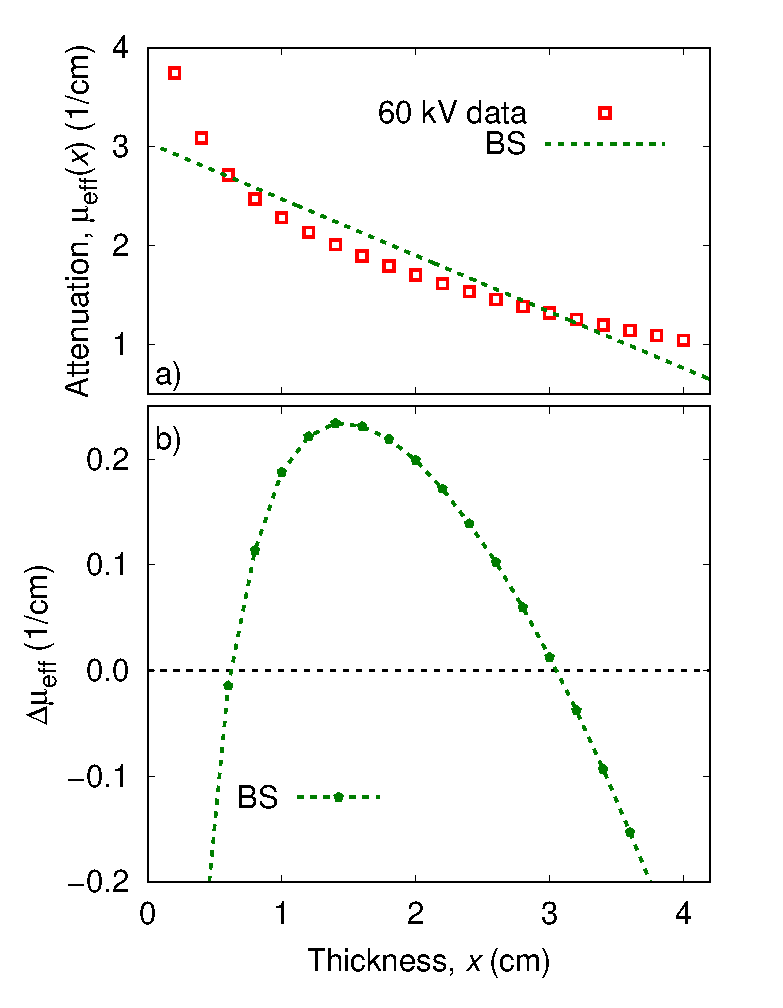
\includegraphics[width=\textwidth]
	{Sources/beam_hardening/borosilicate_glass_60kV_model_comparison_multiplot_2.eps}}
	\only<3>{
	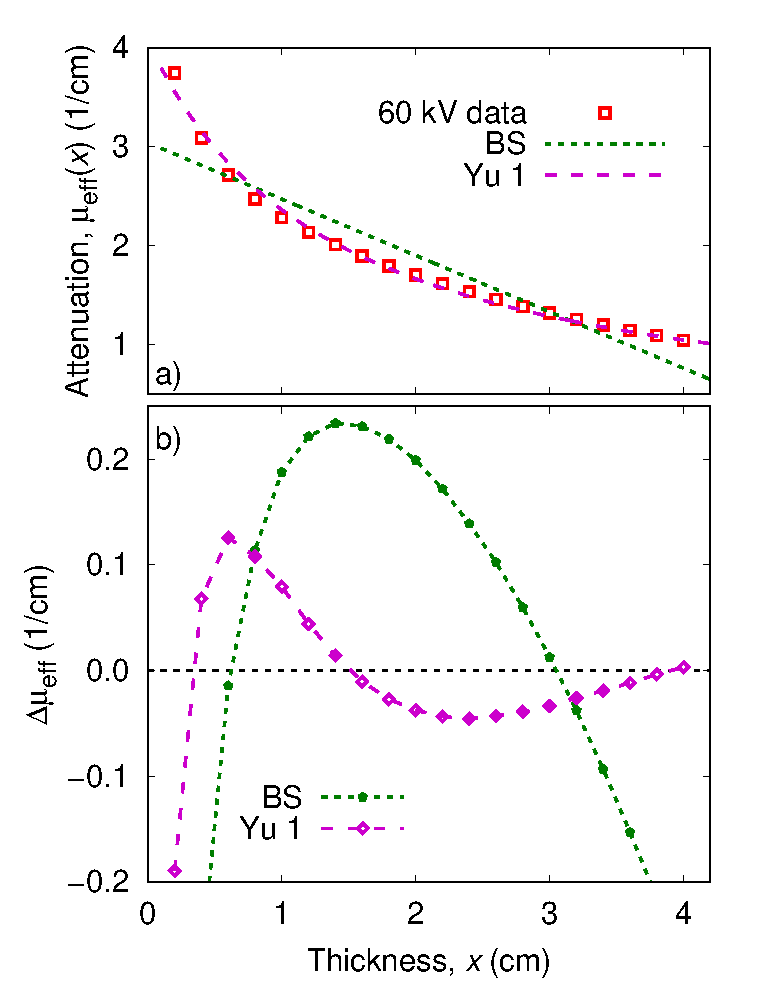
\includegraphics[width=\textwidth]
	{Sources/beam_hardening/borosilicate_glass_60kV_model_comparison_multiplot_3.eps}}
	\only<4>{
	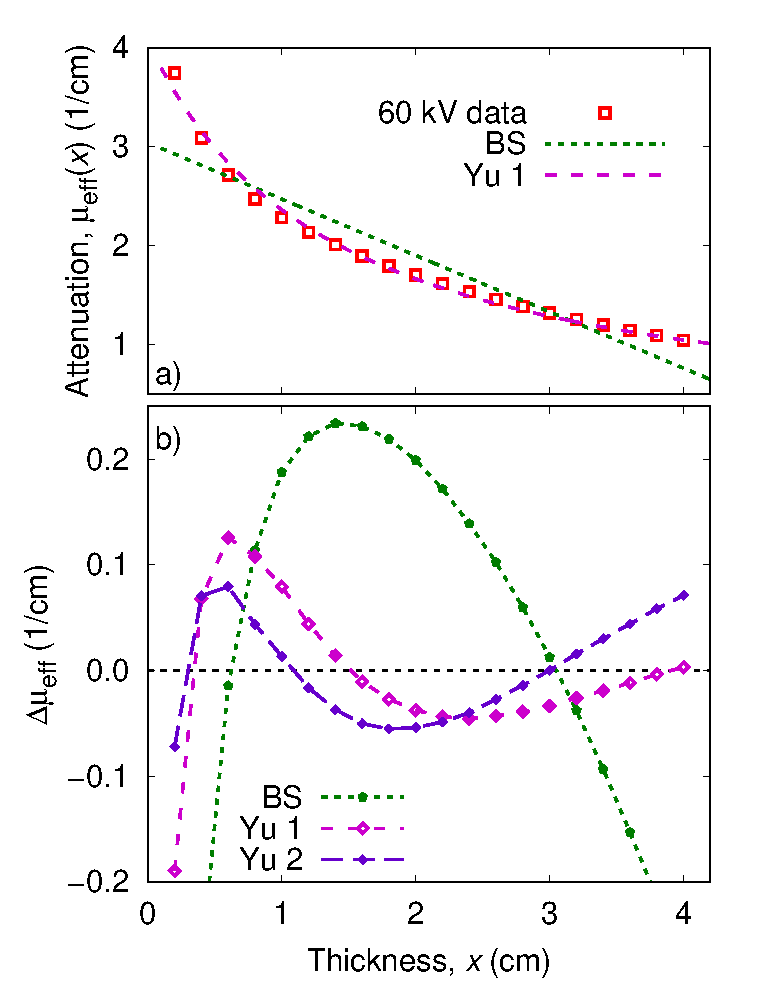
\includegraphics[width=\textwidth]
	{Sources/beam_hardening/borosilicate_glass_60kV_model_comparison_multiplot_4.eps}}
	\only<5>{
	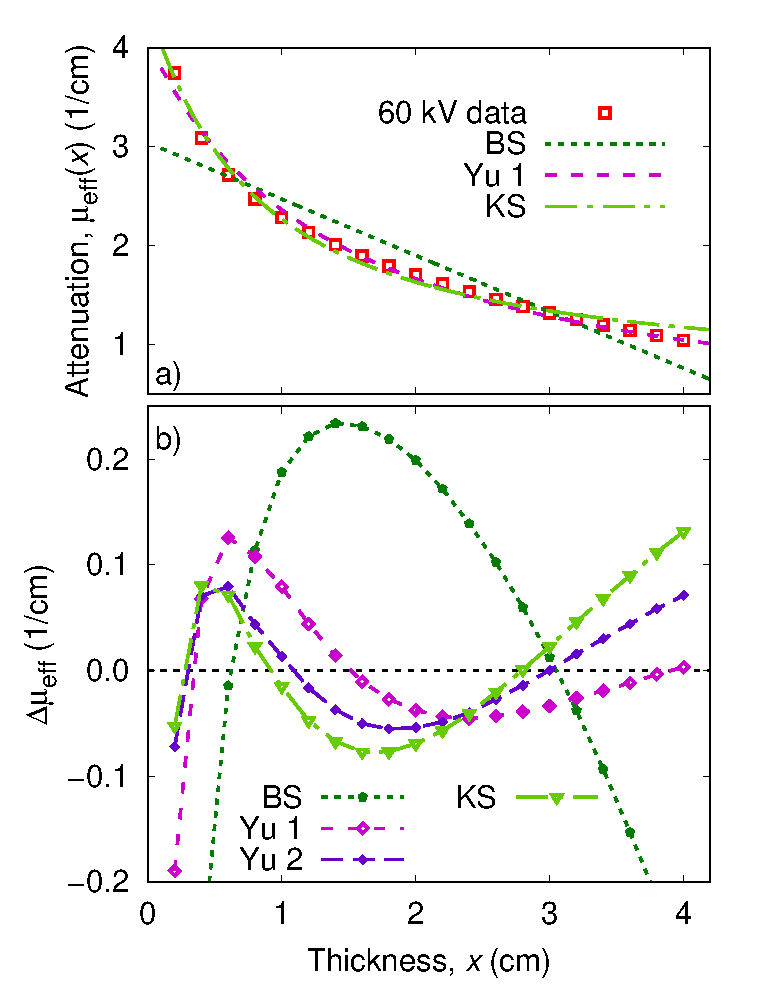
\includegraphics[width=\textwidth]
	{Sources/beam_hardening/borosilicate_glass_60kV_model_comparison_multiplot_5.eps}}
	\only<6>{
	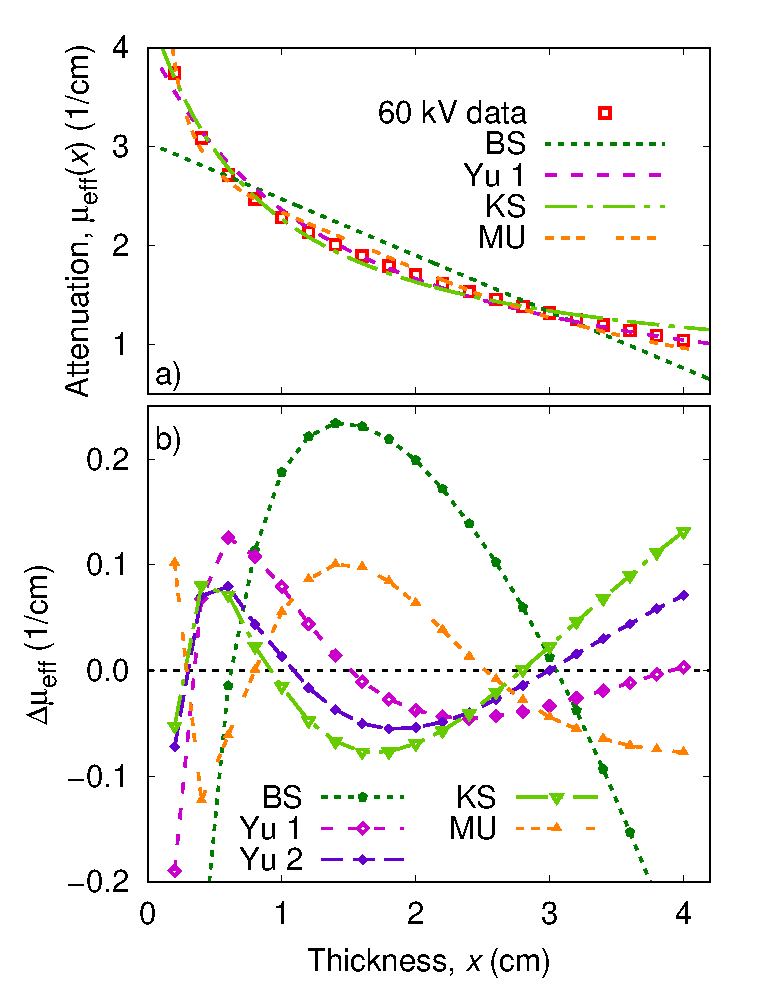
\includegraphics[width=\textwidth]
	{Sources/beam_hardening/borosilicate_glass_60kV_model_comparison_multiplot_6.eps}}
	\visible<7->{
	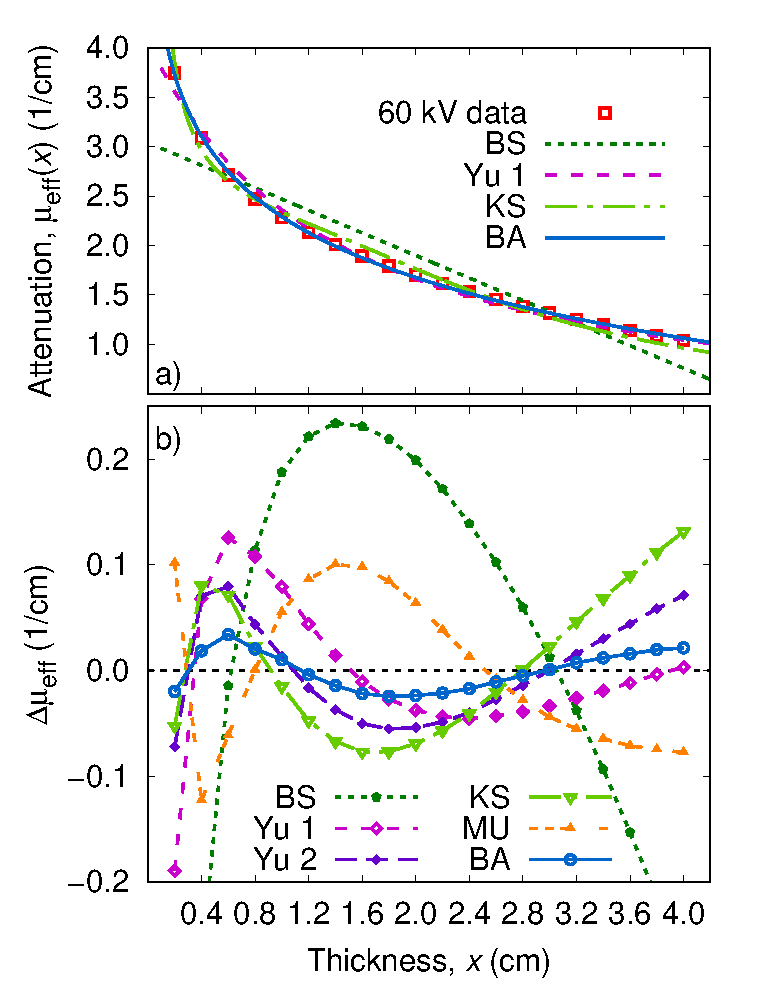
\includegraphics[width=\textwidth]
	{Sources/beam_hardening/borosilicate_glass_60kV_model_comparison_multiplot.eps}}
\end{textblock}


\begin{textblock}{0.5}(0.4, 0.12)
\begin{tabular}{ll}
	\visible<2->{{\small
		\textcolor{BS}{$\mu_\text{eff} (x)= \mu_0 - \lambda x$}} &
	{\small Bjärngard \& Shackford} \\
	& {\small (1994)}\\[0.7cm]}
	
	\visible<3->{
	{\small	
		\textcolor{Yu1}{$\mu_\text{eff}(x) = \frac{\mu_0}{1+\lambda x}$}} &
	\multirow{2}{\linewidth}{\small Yu \textit{et al.} (1997)}\\}
	
	\visible<4->{
	{\small
		\textcolor{Yu2}{$\mu_\text{eff}(x) = \frac{\mu_0}{(1+\lambda x)^\beta}$}} \\[0.7cm]}
	
	\visible<5->{
	{\small
		\textcolor{KS}{
			$\mu_\text{eff}(x) = \mu(E_\text{max}) +
			\frac{2 \mu_1}{x \sqrt{-\lambda_1^2 + 4 \lambda_2}} \times$}} & Kleinschmidt (1999)
	\\
	\multicolumn{2}{l}{\small
		\textcolor{KS}{
			$\quad\left[
			\arctan\left(
			\frac{\lambda_1 + 2 \lambda_2 x}{\sqrt{-\lambda_1^2 + 4 \lambda_2}}
			\right)
			-\arctan\left(
			\frac{\lambda_1}{\sqrt{-\lambda_1^2 + 4 \lambda_2}}
			\right)
			\right]
			$ }} \\[0.7cm]}
	
	\visible<6->{	
	{\small
		\textcolor{MU}{$\mu_\text{eff}(x) = -\frac{1}{x} \ln \left[A+B \exp(-x/C)\right]$}} & 
	{\small
		Mudde \textit{et al.} (2008) }\\[0.7cm]}
	
	\visible<7->{
	{\small
		\colorbox{BA}{\textcolor{white}{{$\boldsymbol{\mu_\text{eff}(x) = a + \frac{b}{x^\alpha}}$}}}} &
	{\small \textbf{Baur \textit{et al.} (2019)}}\\
	& {\small (this work)}}
\end{tabular}
\end{textblock}
}

%% ------------- RESULTS -----------------------------
\frame{
\begin{tikzpicture}[remember picture,overlay]
\fill[blue1]
(current page.north west) rectangle ([xshift=0.22\textwidth,yshift=-10.cm]current page.west|-{pic cs:end});
\end{tikzpicture}

\begin{textblock}{0.2}(0.01,0.15)
	\textcolor{white}{\Large
	{Applicability of }{\large$\boldsymbol{\mu_\text{eff}(x) = a + \frac{b}{x^\alpha}}$}}
\end{textblock}

\begin{textblock}{0.2}(0.005,0.35)
	\centering
	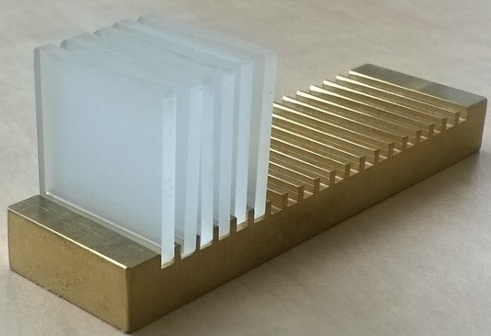
\includegraphics[width=0.8\textwidth]
	{Sources/beam_hardening/plates_on_slide.png}
\end{textblock}

\begin{textblock}{0.2}(0.005,0.65)
	\centering
	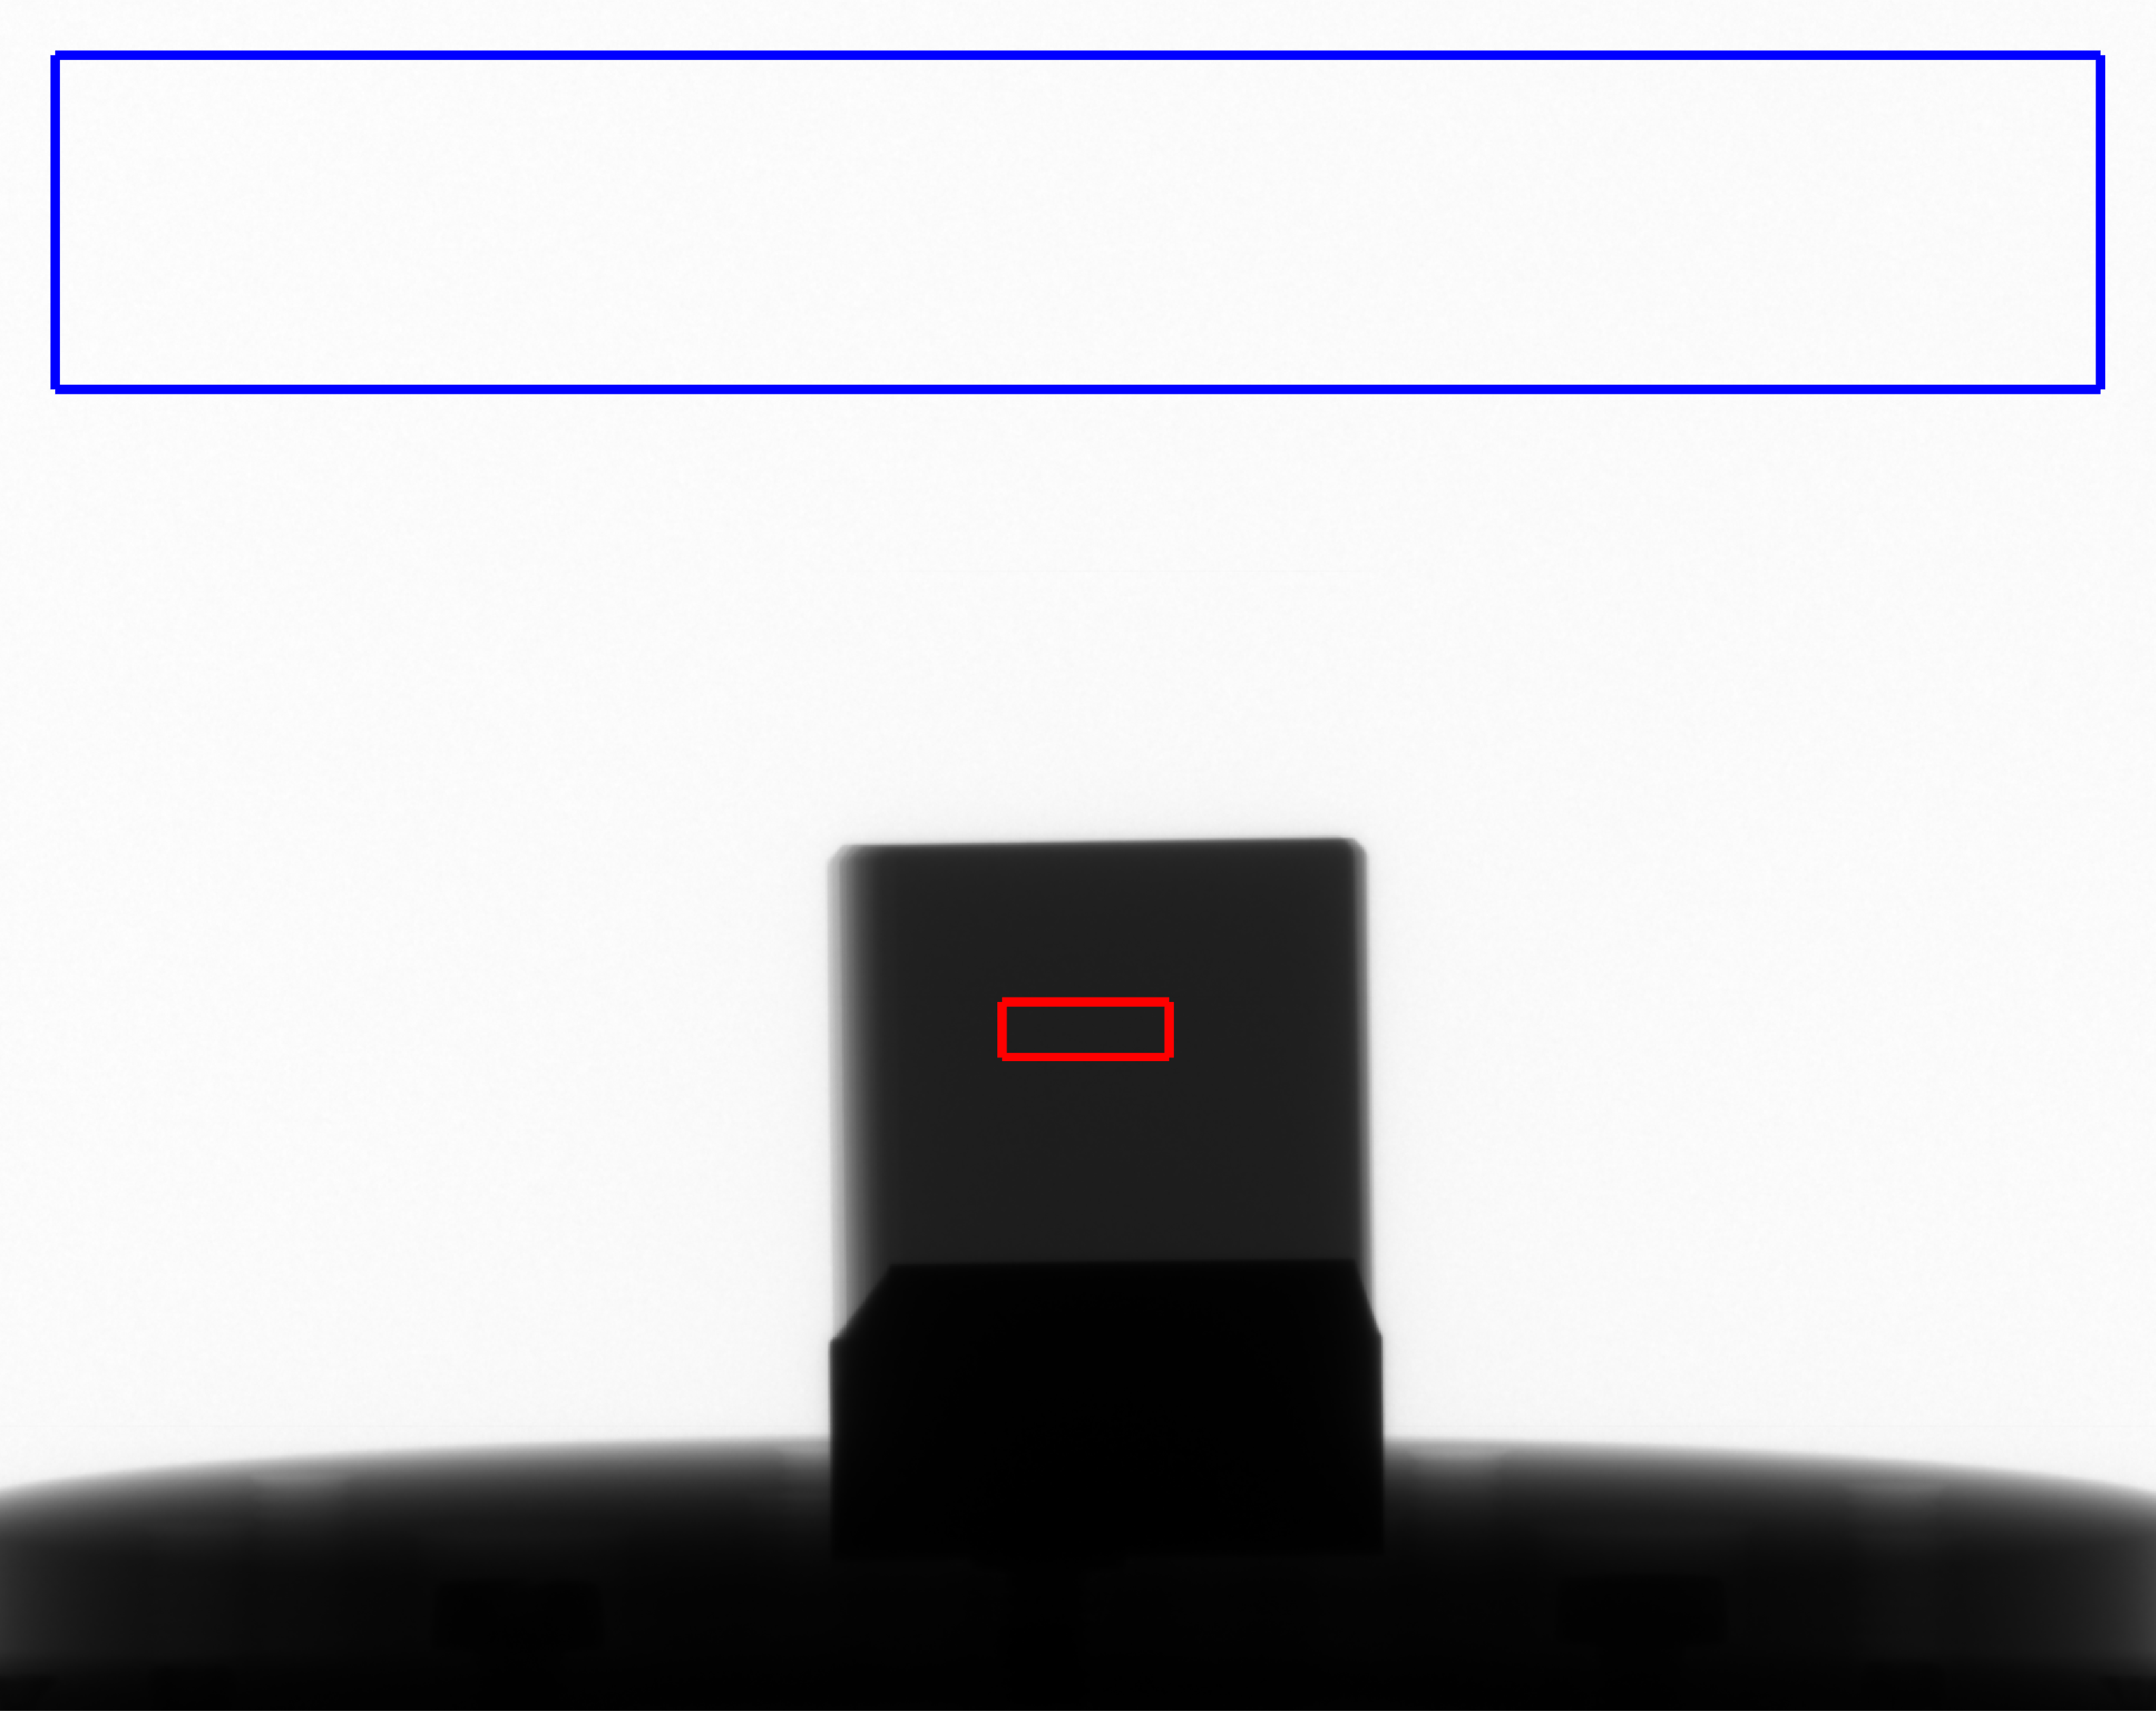
\includegraphics[width=0.8\textwidth]
	{Sources/beam_hardening/20_plates.png}
\end{textblock}



%%% VOLTAGES
\begin{textblock}{0.39}(0.23,0.0)
	\visible<1->{
		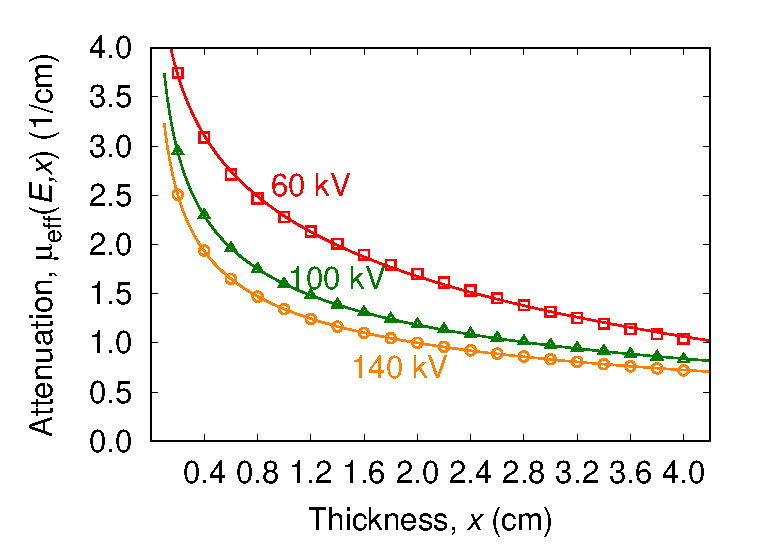
\includegraphics[width=\textwidth]
		{Sources/beam_hardening/borosilicate_glass_voltages_mu_eff.eps}}
\end{textblock}

\begin{textblock}{0.6}(0.23,0.0)
	\vspace{0.5cm}	
	\visible<1->{
		\hspace{3.cm} \colorbox{blue1}{\textcolor{white}{
		 different voltages}}}
\end{textblock}


%% FILTERS
\begin{textblock}{0.39}(0.62,0.0)
	\visible<2->{
		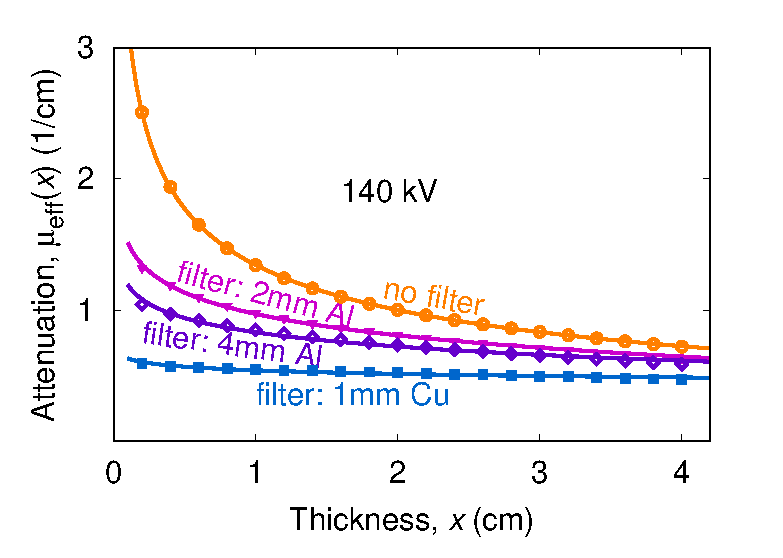
\includegraphics[width=\textwidth]
		{Sources/beam_hardening/borosilicate_glass_filters_mu_eff.eps}}
\end{textblock}

\begin{textblock}{0.6}(0.62,0.0)
	\vspace{0.5cm}	
	\visible<2->{
		\hspace{3.cm} \colorbox{blue1}{\textcolor{white}{
				different filters}}}
\end{textblock}

%% MATERIALS
\begin{textblock}{0.39}(0.23,0.5)
	\visible<3->{
		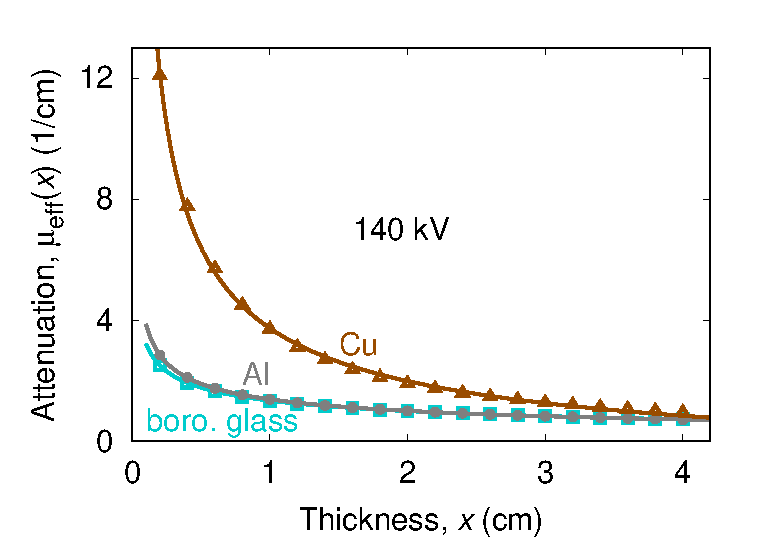
\includegraphics[width=\textwidth]
		{Sources/beam_hardening/materials_mu_eff_140kV_fit.eps}}
\end{textblock}

\begin{textblock}{0.6}(0.23,0.5)
	\vspace{0.5cm}	
	\visible<3->{
		\hspace{3.cm} \colorbox{blue1}{\textcolor{white}{
				different materials}}}
\end{textblock}

%% SETUPS
\begin{textblock}{0.39}(0.62,0.5)
	\visible<4->{
		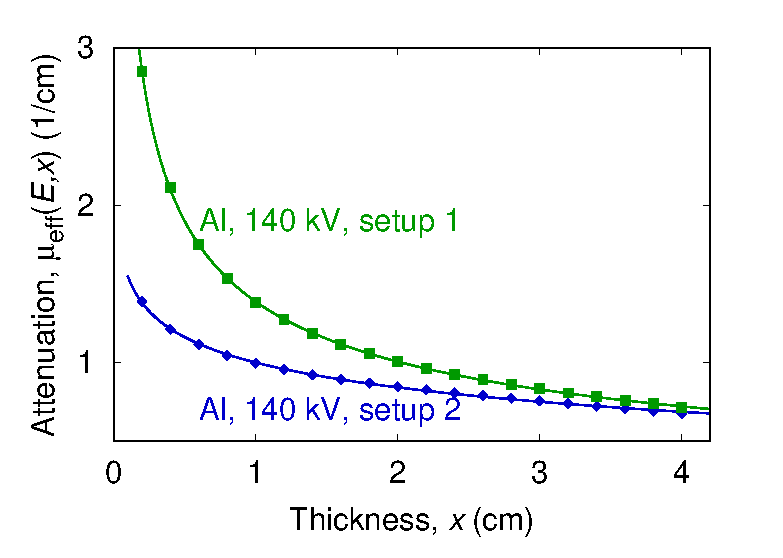
\includegraphics[width=\textwidth]
		{Sources/beam_hardening/comp_both_setups.eps}}
\end{textblock}

\begin{textblock}{0.6}(0.56,0.5)
	\vspace{0.5cm}	
	\visible<4->{
		\hspace{3.cm} \colorbox{blue1}{\textcolor{white}{
				different X-ray setups}}}
\end{textblock}
}

%% ------------- MATERIAL THICKNESS X
\frame{
\begin{tikzpicture}[remember picture,overlay]
\fill[blue1]
(current page.north west) rectangle ([xshift=0.55\textwidth,yshift=0.34\textheight]current page.west|-{pic cs:end});
\end{tikzpicture}

\begin{textblock}{0.5}(0.02,0.03)
	\textcolor{white}{
		\Large Determining the material thickness $x$}
\end{textblock}


\begin{textblock}{0.5}(0.05,0.15)
\visible<1->{
Generalized Beer-Lambert
\[ I(x) = I_0 \exp(-\mu_\text{eff} (x) \, x) \]

Model function
\[ \mu_\text{eff} (x) = a + \frac{b}{x^\alpha} \]\\[0.5cm]
}

\visible<2->{
Solve
\[ a x + b x^{1-\alpha} + \ln \left(\frac{I(x)}{I_0}\right) = 0\]
e.g.\ Newton's method or look-up table}
\end{textblock}

\begin{textblock}{0.48}(0.48,0.05)
\only<1>{
	\includegraphics[width=\textwidth]
	{Sources/beam_hardening/3datapoints_top.eps}
}

\only<2>{
	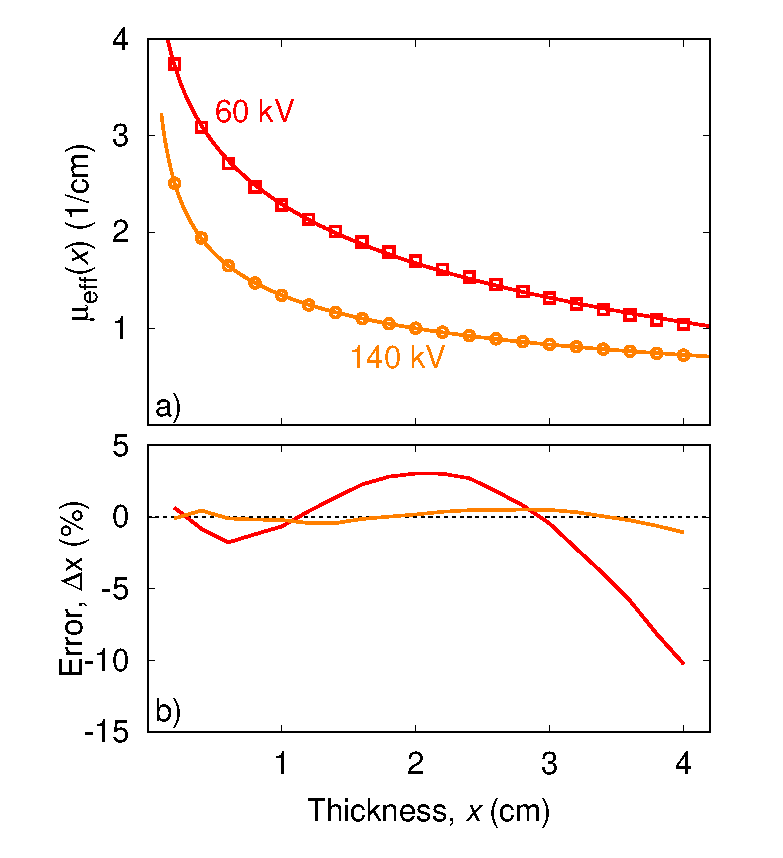
\includegraphics[width=\textwidth]
	{Sources/beam_hardening/3datapoints_top_bottom.eps}
}

\visible<3->{
	\includegraphics[width=\textwidth]
	{Sources/beam_hardening/3datapoints_final.eps}
}
\end{textblock}
}

%% ------------- Applications ------------------------
\frame{
\begin{tikzpicture}[remember picture,overlay]
\fill[blue1]
(current page.north west) rectangle ([xshift=1.\paperwidth,yshift=0.33\paperheight]current page.west|-{pic cs:end});
\end{tikzpicture}

\begin{textblock}{1.}(0.02,0.03)
	\textcolor{white}{
		\Large Migrating shear bands in shaken granular matter, Kollmer \textit{et al} (2020)}
\end{textblock}

\begin{textblock}{0.9}(0.05,0.12)
	\centering
	\only<1>{
	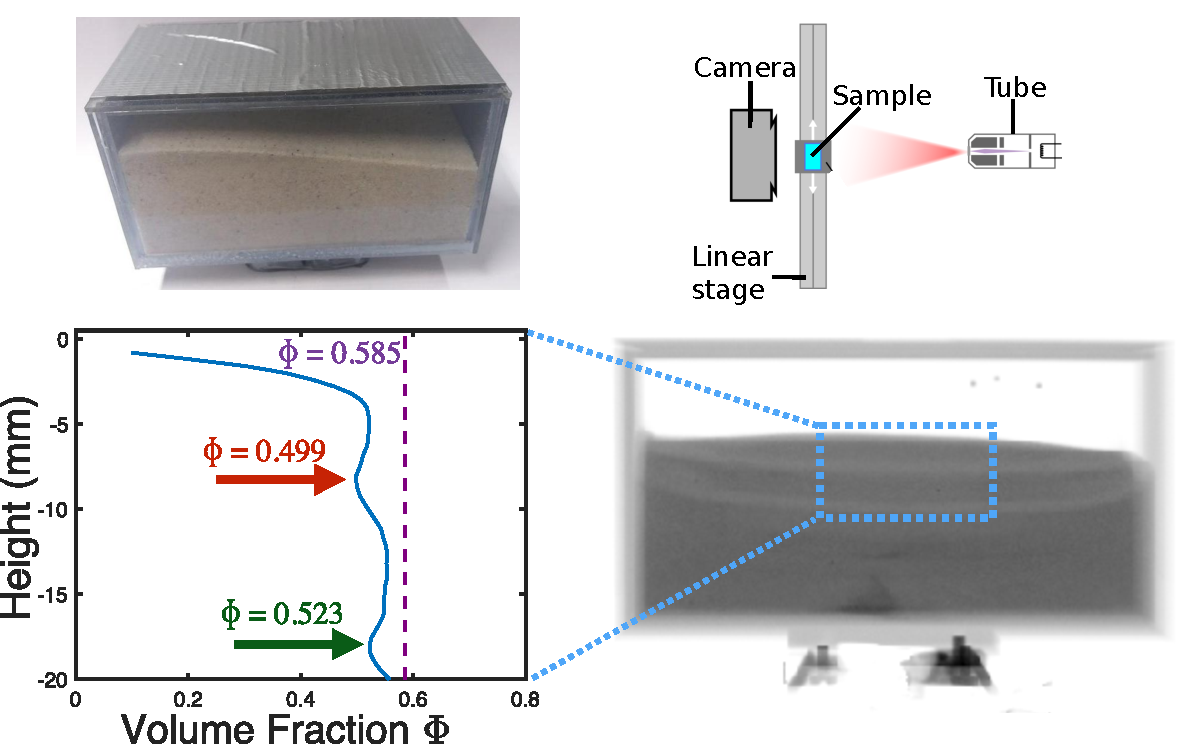
\includegraphics[width=0.8\textwidth]
	{Sources/beam_hardening/migrating_shearband.pdf}}
\end{textblock}
}